In this section, we first describe our experimental setup concerning both the instances we use as a benchmark as well as the hardware in use in \ref{eval: setup}.
\todo{rest of the stuff }

\subsection{Experimental Setup}
\label{eval: setup}
For our performance tests we utilize the same reduced IPC 2020 benchmark as in \cite{bretl2021parallel}, also giving our planners 900 seconds per instance. \\
The performance tests were done on a server with an Intel Xeon Gold 6138 processor with 4 sockets, 20 cores per socket and 2 threads per core clocked 2.00G Hz with around 750GB of RAM and running Ubuntu 20.04.\\
We performed an additional test with an instrumented version of single-threaded CrowdHTN using random DFS and hash set based loop detection. The instrumentation allowed us to track information on the structure of our search graph and planner behavior, such as the prevalence of loops and search nodes created per second. This run was performed on the same set of instances as the performance test with up to 300 seconds per instance. The investigation was performed on a server with an AMD EPYC 7702 processor with 1 socket with 64 cores and 2 threads per core clocked 2.00 GHz with around 1TB of RAM and running Ubuntu 20.04. \\
\todo{describe machine used in malleability tests}

\begin{comment}
CrowdHTN metadata
- same instance set
- 300 seconds per instance
- log the run time behavior regarding the search behavior
- 64 cores, 2 GHz max
- AMD EPYC 7702
- around 1 TB of RAM
- Ubuntu 20.04
\end{comment}

\subsection{Optimizations in CrowdHTN}
\label{eval: crowd optimizations}
- putting numbers to memory savings and how many nodes we save from instantiation (also saves our loop detection!)
- percentage of search nodes saved by not representing search nodes beginning with an action
- percentage of world states saved by sharing them between nodes

\subsection{Search Algorithms}
\label{eval: algorithms}
In section \ref{improv: search algorithms} we presented four search algorithms that we implemented for CrowdHTN. Those algorithms are random DFS, heuristic DFS, A-star like and BFS. We have tested all four algorithms on our test instance set using 4 PEs and a local bloom filter without restarts for loop detection. The results of this test are visualized in figure \ref{figure: eval algorithm}, a summary of coverage and IPC score is presented in table \ref{table: eval algorithm}. \\
Overall, random DFS performed best, followed by heuristic DFS, A-star like search and finally BFS with our best algorithm, random DFS, solving almost twice as many instances and having twice the IPC score of our worst algorithm, BFS. Additionally, we observe a hit-or-miss behavior in both our DFS implementations where plans are either found almost immediately or not at all. Out of the 50 instances solved by random DFS, only 18 were solved in more than 1 and out of these 18 only 9 were solved in more than 10 seconds. BFS on the other hand solves 14 out of 30 instances in more than a second and 11 of these 14 in over 10 seconds. As such, while overall worse performing it does seem to scale better with runtime. \\
Comparing our two DFS-based approaches, we see that random DFS performs better than heuristic DFS guided by our heuristic from section \ref{improv: crowd heuristic}. We attribute this to the fact that we consciously limited our heuristic to information on the hierarchy available from the lifted instance to reduce the time spent on precomputation. Others, such as \cite{holler2020htn} argue that heuristics must utilize both hierarchy and world state information. Our findings corroborate this theory.

\begin{figure}
	\caption{Plotting the number of solved instances per run time for CrowdHTN using DFS, heuristic DFS, A-star like search and BFS}
	\label{figure: eval algorithm}
	\centering
	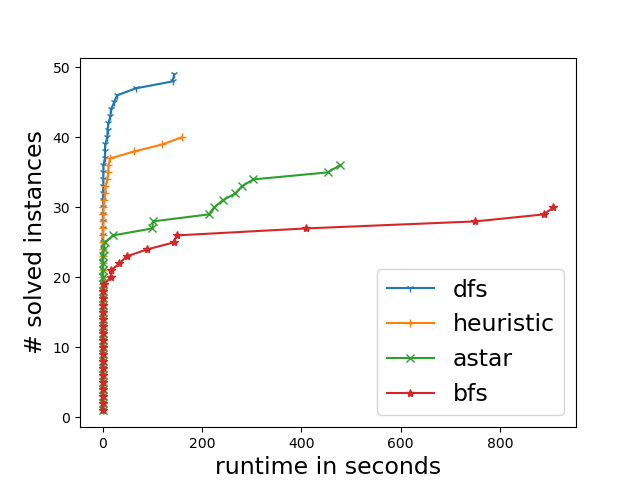
\includegraphics[width=0.5\textwidth]{images/final/search_algorithms.png}
\end{figure}
\begin{table}
	\caption{Coverage and IPC score of our search algorithms using 4 PEs and a local bloom filter}
	\label{table: eval algorithm}
	\centering
	\begin{tabular}{| l | r | r |}
		\hline
		Algorithm 		& Coverage & IPC Score \\
		\hline
		Random DFS 		& 41.7\%	& 43.09 \\ % 50
		Heuristic DFS 	& 33.3\%	& 35.60	\\ % 40
		A-star like 	& 38.3\%	& 27.13 \\ % 36
		BFS 			& 25.0\%	& 21.87	\\ % 30
		\hline
	\end{tabular}
\end{table}

\subsection{Scalability of Parallel CrowdHTN}
\label{eval: scalability}
- show scaling on a nice instance

\begin{figure}
	\caption{Plotting the number of solved instances per run time for CrowdHTN using DFS and a local bloom filter on 64, 16 and 4 PEs}
	\label{figure: eval scalability}
	\centering
	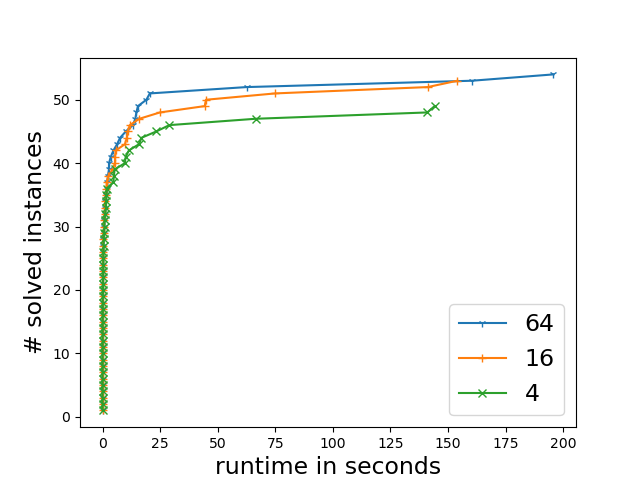
\includegraphics[width=0.5\textwidth]{images/final/scalability}
	% python3 ../MA_scripts/diagrams.py -files=results_64_dfs_local_bloom.csv,results_16_dfs_local_bloom.csv,results_4_dfs_local_bloom.csv  -names=64,16,4
\end{figure}

\subsection{Loop Detection}
\label{eval: loop detection}
- general loop detection:
- loop hit rate
- global loop hit rate
- performance of hash set vs bloom filter

- add runs without any loop detection to the evaluation
- split perf comparison on domains with and without loops
- table which gives us domain and loop percentage

\begin{figure}
	\caption{Plotting the number of solved instances per run time for CrowdHTN comparing hash set and local bloom filter based loop detection on 32 and 64 PEs}
	\label{figure: eval loop detection}
	\centering
	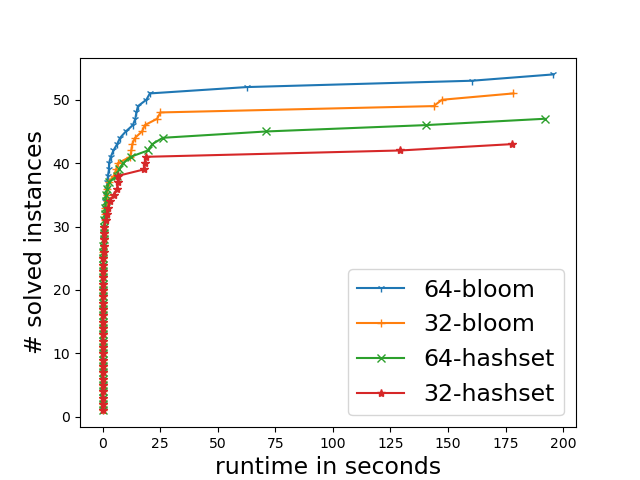
\includegraphics[width=0.5\textwidth]{images/final/loop_detection}
	% python3 ../MA_scripts/diagrams.py -files=results_64_dfs_local_bloom_handlepanic_1.csv,results_32_dfs_local_bloom_handlepanic.csv,results_64_dfs_local_hashset_handlepanic.csv,results_32_dfs_local_hashset_handlepanic.csv -names=64-bloom,32-bloom,64-hashset,32-hashset
\end{figure}

\begin{table}
	\caption{Coverage and IPC score while using hash set and local bloom filter based loop detection on 32 and 64 PEs}
	\label{table: eval loop detection}
	\centering
	\begin{tabular}{| l | r | r |}
		\hline
		Configuration & Coverage & IPC Score \\
		\hline
		Bloom, 64 PEs		& 45.0\%	& 47.37 \\ % 54
		Bloom, 32 PEs		& 42.5\%	& 44.24 \\ % 51
		Hash set, 64 PEs	& 39.2\%	& 41.84 \\ % 47
		Hash set, 32 PEs	& 35.8\%	& 38.71 \\ % 43
		\hline
	\end{tabular}
\end{table}

\subsection{Probabilistic Restarts}
\label{eval: restarts}
- test the probabilistic restarts
- with 900 seconds we expect $\sum_{t=1}^{899} \frac{1}{t} \approx 7.38$ restarts per run


\subsection{Global Loop Detection}
\label{eval: global loop}
- test the global loop detection

\subsection{Malleable CrowdHTN}
\label{eval: malleable}
- test the malleability

\subsection{Conclusion}
\label{eval: conclusion}
- final discussion stuff
